
\documentclass[11pt, a4paper]{article}
%\usepackage{proj1}
\usepackage{natbib}
\usepackage{fancyhdr}  
\usepackage{subcaption}
\usepackage{caption}
\usepackage{graphicx}
\usepackage{numprint}
\usepackage{multirow}
\linespread{1.25} 
\setlength{\parindent}{0cm}
\graphicspath{{Images/}}
\usepackage{hyperref}
\usepackage{amsmath}
\usepackage{amsfonts}
\usepackage{amssymb}
\usepackage{amsthm}
\usepackage{mathtools}
\usepackage{commath}
\usepackage{bbm}

%\usepackage[sc,osf]{mathpazo}
\usepackage{subcaption}
\usepackage[a4paper, top=1in, left=1.0in, right=1.0in, bottom=1in, includehead, includefoot]{geometry} %Usually have top as 1in

\usepackage{listings}
\usepackage{color} %red, green, blue, yellow, cyan, magenta, black, white
\definecolor{mygreen}{RGB}{28,172,0} % color values Red, Green, Blue
\definecolor{mylilas}{RGB}{170,55,241}


\hypersetup{colorlinks,linkcolor={black},citecolor={blue},urlcolor={black}}
\usepackage{color}
\urlstyle{same}


\theoremstyle{definition}
\newtheorem{definition}{Definition}[section]

\newcommand{\adja}{q_a}
\newcommand{\adjb}{q_b}
\newcommand{\adjaB}{q_{a,\partial \Omega}}
\newcommand{\adjbB}{q_{b,\partial \Omega}}
\newcommand{\adjB}{q_{\partial \Omega}}
\newcommand{\Adja}{\mathbf{p}}
\newcommand{\Adjb}{q}
\newcommand{\adj}{q}
\newcommand{\Adjc}{{q}_{\partial \Omega}}
\newcommand{\ra}{\rho_a}
\newcommand{\rb}{\rho_b}
\newcommand{\w}{\mathbf{w}}
\newcommand{\x}{\mathbf{x}}
\newcommand{\f}{\mathbf{f}}
\newcommand{\ve}{\mathbf{v}}
\newcommand{\n}{\mathbf{n}}
\newcommand{\h}{\mathbf{h}}
\newcommand{\K}{\mathbf{K}}
\newcommand{\hr}{\widehat \rho}
\newcommand{\jf}{\mathbf j}

\DeclareMathOperator{\sgn}{sgn}
\DeclareMathOperator{\Grad}{Grad}
\DeclareMathOperator{\Div}{Div}
\DeclareMathOperator{\Lap}{Lap}
%	\begin{figure}[h]
%		\centering
%		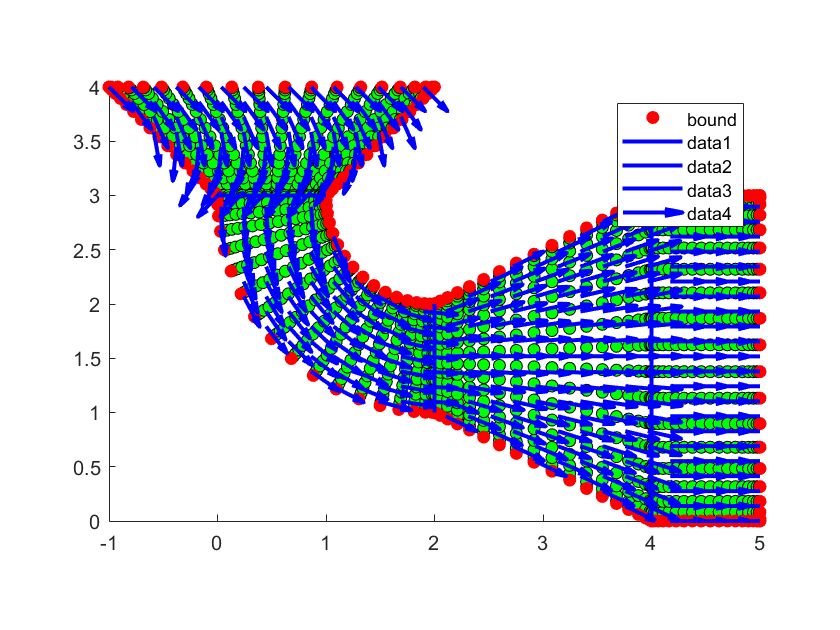
\includegraphics[scale=0.35]{F1.png}
%		\caption{Forward $\rho$ for $a = 0.01$} 
%		\label{F1}
%	\end{figure}

\begin{document}
Annual Review (in particular structure) and Extension Request.\\
Paper: added required terms, code snippet. Too long?
\section{Newton-Krylov Investigation}
\subsection{'Final time independent' solutions}
We investigate whether the time scaling has an effect on the odd behaviour of the Neumann exact solution.
We choose the following inputs
\begin{align*}
	\rho &= 0.25\beta^{1/2}\exp(t/T) (\cos(\pi x) + 1), \\
	q &= 0.25\beta^{1/2}(\exp(T/T) - \exp(t/T))\cos(\pi x) 
\end{align*}
For $n = 10$, $N = 30$, we have for $T = 1$, the exact error for $\rho$ and $q$ is of order $10^{-15}$ and $10^{-14}$, for $T = 5$, we get an error of $10^{-14}$ and $10^{-13}$ respectively. For $T= 0.1$ we get errors of order $10^{-15}$.
For $n = 20$, $N = 30$ , for $T = 1$ we have errors of order $10^{-15}$, for $T = 5$, the error is $10^{-14}$ and $10^{-13}$ and for $T = 0.1$ we only get $10^{-6}$.\\
For $n = 25$, $N = 30$, for $T = 1$ we only get $10^{-7}$/ $10^{-6}$ accuracy, while for $T = 5$, we get $10^{-14}$ (ans for $T = 0.1$ we only get $10^{-3}$/$10^{-4}$). This is not changed by increasing $N$ to $40$.
For $n = 30$, $N = 40$, $T = 5$ is also not that accurate anymore, and only $T = 20$ results in $10^{-11}$/$10^{-9}$. For $N = 35$ it improves to $10^{-13}$.

\subsection{Perturbation in Time}
We take the perturbation from the second year review.
We consider multiplying the exact solution by $1+ \epsilon p(t)$, where $p(t)$ is the perturbation at time $t$. For $\epsilon  = 0$ , the algorithm converges immediately. For $n = 30$, $N = 35$, for $\epsilon = 0.0001$ we get an error of $10^{-7}$ and the algorithm reaches $100$ inner iterations each time. For $\epsilon = 0.01$ we get errors of $10^{-5}$.
For $n = 20$ and $N = 30$, we get $10^{-15}$, even for $\epsilon = 0.1$. So this suggests that the time scaling thing from the previous section is more of a problem.

\subsection{Increasing number of iterations}
However, if we instead increase the maximum number of iterations, this also improves convergence. For $n = 30$, $N = 35$, we get for $\epsilon = 0.01$, instead of an error of $10^{-5}$, with max $200$ iterations we get an error of $10^{-14}$. The same result holds for $\epsilon = 0.1$.
\\
\\
We investigate the same relationship between maximum iterations and time scaling. Giving again the initial conditions as initial guess, we get for $n = 30$ and $N = 35$, for $T = 1$ with $20$ iterations we get an error of $10^{-14}$ instead of $10^{-3}$. The inner iteration still reaches this maximum sometimes, but not each time as is the case for $100$ maximum iterations.
For $T = 0.1$ we improve to $10^{-8}$, but reach the maximum iterations often. For maximum of $300$ iterations, we get down to $10^{-15}$.
\\
\\
So overall I would conclude that some things are harder and therefore need more inner iterations.
\\
\\
The issue with $T = 0.1$ and $n = 30$/ $N = 35$ can be observed for the Dirichlet problem, too. However, the solution is still $10^{-8}$ accurate (as opposed to $10^{-3}$ for Neumann). Increasing the number of iterations to $200$, we get $10^{-15}$ accuracy. For $T = 1$, we don't have a problem for Dirichlet.\\
For the perturbation with $n = 30$ and $N = 35$ we don't have a problem, even for large $\epsilon$, which makes sense because this is computed at $T = 1$, which didn't cause problems for the initial condition as initial guess (which is further from the exact solution than the perturbed problem).\\
\\
\\
Increasing the number of iterations does not improve the difference in the paper example (between Newton-Krylov and Fixed Point Algorithms). The error between the two approaches furthermore is consistent for different values of $\beta$.
\section{Comparing Fixed Point with Newton-Krylov (from last week - for reference)}
\subsection{1D Problems}
I apply this observation to one of the paper examples (Example 2), with $\kappa = 1$. When I run the problem with $N = 50$ and $n = 10$, and then with the old code with $n = 30$ and interpolate to $n = 10$ in time, We get an error of $0.0362$. If I run both versions with $n = 30$ we get an error of $3.8640 \times 10^{-4}$, which seems to contradict the above observation. \\
For $n = 30$, we get for $\kappa =-1$ and error of $0.0013$ and for $\kappa = 0$ and error of $1.2519 \times 10^{-8}$. These problems take $56$ seconds to solve.
\\
\\
For the paper example 1, we again choose $N = 50$ and $n = 30$. We get for $\kappa = 0$ an error of $1.5563 \times 10^{-13}$, for $\kappa = -1$ we have the error $0.0174$ and for $\kappa = 1$, the error is $0.0037$. The same error results from comparing NK to fsolve for this problem set up with $n = 20$, $N = 30$. The error between fixed point and fsolve is of order $10^{-7}$.
	\begin{figure}[h]
		\centering
		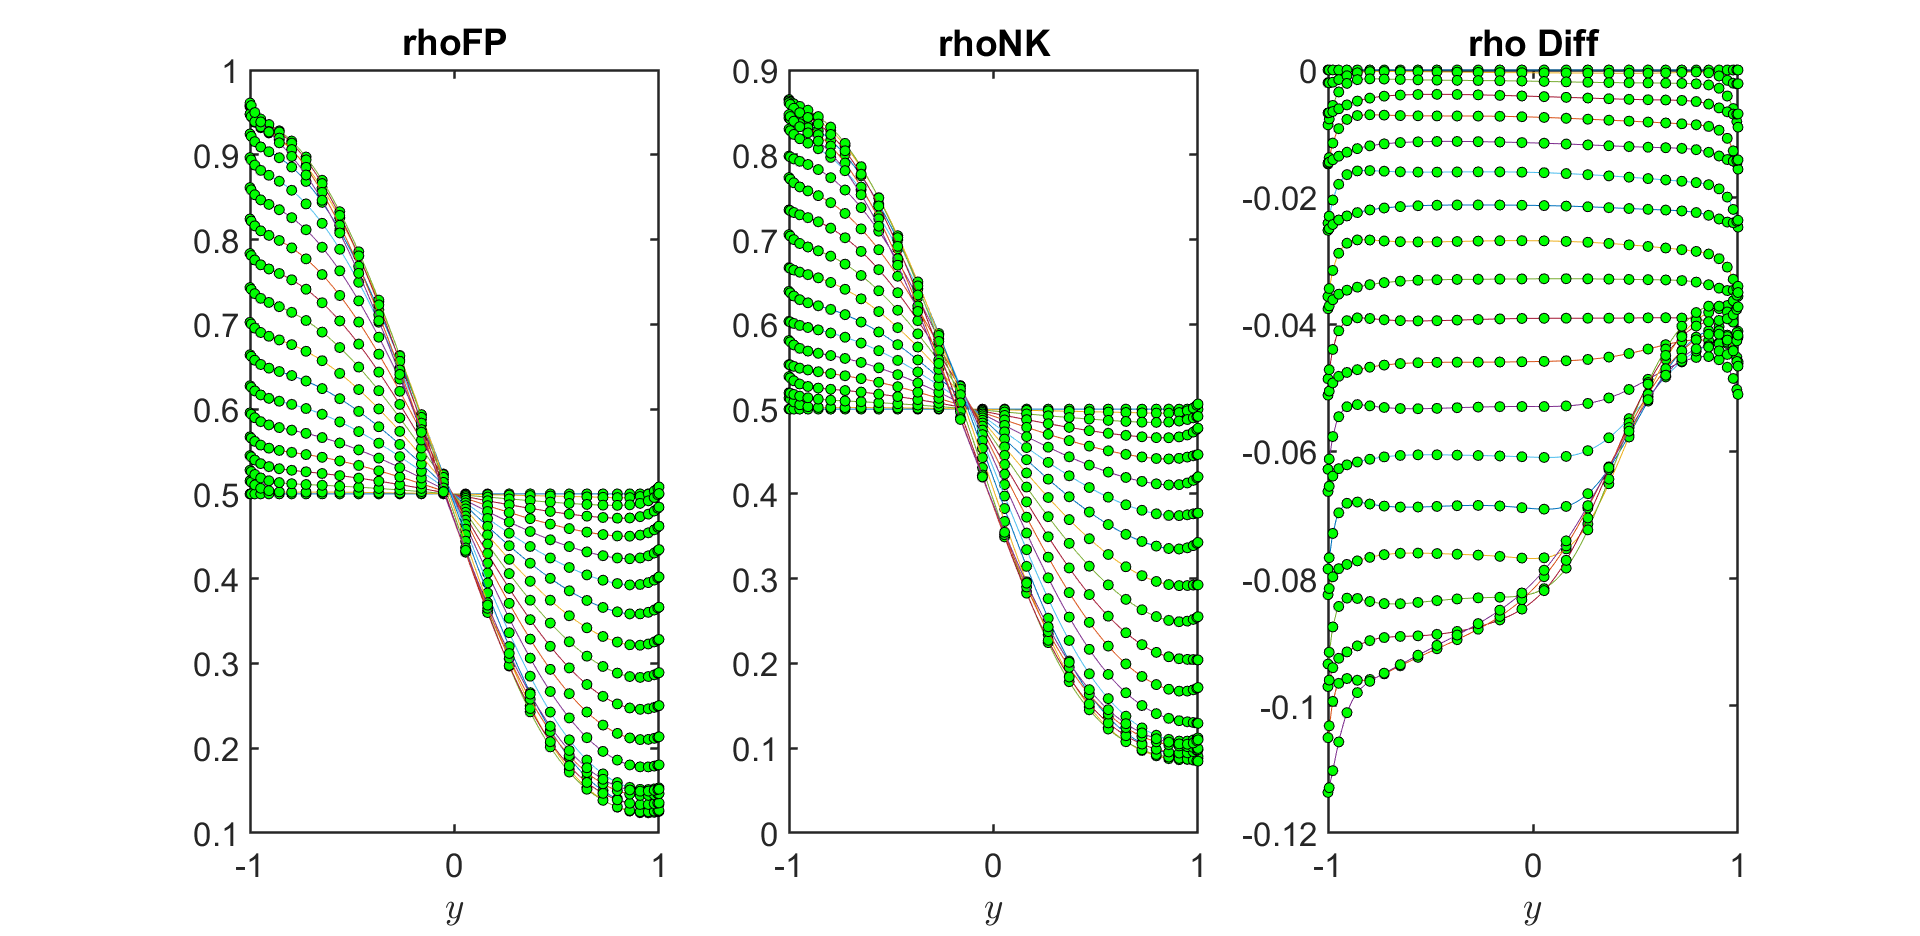
\includegraphics[scale=0.35]{Ex1.png}
		\caption{Paper Example 1 with $\kappa = 1$, $n = 20$, $N = 30$, Comparison between fix point and Newton Krylov} 
		\label{F1}
	\end{figure}
\\
\\
For the third example, we have Dirichlet BCs and again choose $N = 50$ and $n = 30$. We get for $\kappa = 0$ the eroor is $1.8015 \times 10^{-7}$, for $\kappa = -1$ the error is $1.6645 \times 10^{-7}$ and for $\kappa  =1$ the error is $1.9485 \times 10^{-7}$.


\subsection{2D Problems}
The exact 2D Dirichlet problem (with and without external potential), for $N = 20$ and $n = 10$, has an error of $10^{-15}$ for both $u$ and $v$ and is solved in $40$ and $60$ seconds respectively. The exact Neumann problem reduces the error in $u$ to $10^{-8}$ and in $v$ to $10^{-7}$. The inner iterations reach $100$ and it takes $170$ seconds.
For the first paper problem, we have the following results. For $\kappa = -1$ the error is $0.0032$, for $\kappa = 0$, the error is $3.6813 \times 10^{-9}$ and for $\kappa = 1$ the error is $0.0014$.
For the second paper problem, we have the following results. For $\kappa = -1$ the error is $0.0062$, for $\kappa = 0$, the error is $3.1640 \times 10^{-4}$ and for $\kappa = 1$ the error is $0.0017$.
All of these problems take $300$ to $500$ seconds.



\section{Curl free control}	
We consider
\begin{align*}
	&\min_{\rho, \w} \frac{1}{2}\int_0^T \int_\Omega \left(\rho - \hr\right)^2 d\x dt + \frac{\beta}{2}\int_0^T \int_\Omega \w^2 d\x dt + \frac{\eta}{2}\int_0^T \int_\Omega \left(\nabla \times \w \right)^2 d\x dt\\
	&\text{subject to:}\\
	& \frac{\partial \rho}{\partial t} = \nabla^2 \rho - \nabla \cdot \left(\rho \w\right)\\
	& \frac{\partial \rho}{\partial n} - \rho \w \cdot \n = 0
\end{align*}
We know that in two dimensions
\begin{align*}
    \nabla \times \w = \frac{\partial w_2}{\partial x_1}  - \frac{\partial w_1}{\partial x_2}.
\end{align*}
More importantly, we know that
\begin{align}\label{eqn:CurlRel}
	\nabla \times \w = \nabla \cdot  \w_\bot,
\end{align}
where $\w_\bot = (w_2 , -w_1)$, the result of a rotation of $\w$ by $\pi/2$.
Then the Lagrangian is
\begin{align*}
	\mathcal L (\rho, \w ,q_1, q_2) =& \frac{1}{2}\int_0^T \int_\Omega \left(\rho - \hr\right)^2 d\x dt + \frac{\beta}{2}\int_0^T \int_\Omega \w^2 d\x dt + \frac{\eta}{2}\int_0^T \int_\Omega \left(\nabla \cdot  \w_\bot \right)^2 d\x dt\\
	&- \int_0^T \int_\Omega q_1 \left(\frac{\partial \rho}{\partial t} - \nabla^2 \rho + \nabla \cdot \left(\rho \w\right) \right) d \x dt \\
	&- \int_0^T \int_{\partial \Omega} q_2\left(\frac{\partial \rho}{\partial n} - \rho \w \cdot \n \right) d\x dt.
\end{align*}
Then, since we know that $q_1 = q_2$, we get
\begin{align*}
	\mathcal L (\rho, \w ,q) =& \frac{1}{2}\int_0^T \int_\Omega \left(\rho - \hr\right)^2 d\x dt + \frac{\beta}{2}\int_0^T \int_\Omega \w^2 d\x dt + \frac{\eta}{2}\int_0^T \int_\Omega \left(\nabla \cdot  \w_\bot\right)^2 d\x dt\\
	&- \int_0^T \int_\Omega -\rho\frac{\partial q}{\partial t} - \rho \nabla^2 q - \nabla q \cdot \left(\rho \w\right) d \x dt  - \int_\Omega q(T) \rho(T) - q(0) \rho(0) d\x\\
	&- \int_0^T \int_{\partial \Omega}  - \rho \nabla q \cdot \n  d\x dt.
\end{align*}
For the adjoint equation, we find the usual results.
We take the derivative with respect to $\w$
\begin{align*}
	\mathcal L_\w(\rho, \w, q)h &= \int_0^T \int_\Omega \beta \w \cdot  \h + \rho \nabla q \cdot \h + \eta \left(\nabla \cdot  \h_\bot\right) \left(\nabla \cdot  \w_\bot\right)d\x dt.
\end{align*}
Then we integrate by parts (or divergence theorem) to get
\begin{align*}
	\mathcal L_\w(\rho, \w, q)h &= \int_0^T \int_\Omega \beta \w \cdot  \h + \rho \nabla q \cdot \h - \eta \nabla\left(\nabla \cdot  \w_\bot\right)  \cdot \h_\bot d\x dt + \int_0^T \int_{\partial \Omega} \eta \left(\nabla \cdot  \w_\bot\right) \h_\bot \cdot \n d \x dt.
\end{align*}
Finally we need to rewrite the equations in terms of $\h$. We note that 
\begin{align*}
	\begin{pmatrix}
		0 & 1\\
		-1 & 0
	\end{pmatrix} 
\h
= 
\h_\bot.
\end{align*}
Furthermore,
\begin{align*}
	\begin{pmatrix}
		0 & -1\\
		1 & 0
	\end{pmatrix} 
	\n \cdot \h
	= 
	\h_\bot \cdot \n.
\end{align*}
Replacing these in the Lagrangian gives
\begin{align*}
	\mathcal L_\w(\rho, \w, q)h &= \int_0^T \int_\Omega \beta \w \cdot  \h + \rho \nabla q \cdot \h - \eta 	\begin{pmatrix}
		0 & -1\\
		1 & 0
	\end{pmatrix} \nabla\left(\nabla \cdot  \w_\bot\right)  \cdot
	\h d\x dt \\
	&+ \int_0^T \int_{\partial \Omega} \eta \left(\nabla \cdot  \w_\bot\right) \begin{pmatrix}
		0 & -1\\
		1 & 0
	\end{pmatrix} 
	\n \cdot \h d \x dt.
\end{align*}
Finally, using \eqref{eqn:CurlRel} we get
\begin{align*}
	\mathcal L_\w(\rho, \w, q)h &= \int_0^T \int_\Omega \beta \w \cdot  \h + \rho \nabla q \cdot \h - \eta 	\begin{pmatrix}
		0 & -1\\
		1 & 0
	\end{pmatrix} \nabla\left(\nabla \times  \w\right)  \cdot
	\h d\x dt \\
	&+ \int_0^T \int_{\partial \Omega} \eta \left(\nabla \times \w\right) \begin{pmatrix}
		0 & -1\\
		1 & 0
	\end{pmatrix} 
	\n \cdot \h d \x dt.
\end{align*}
Since this holds for all admissible $\h$ we get the gradient equation
\begin{align*}
	 \beta \w  + \rho \nabla q - \eta 	\begin{pmatrix}
	 	0 & -1\\
	 	1 & 0
	 \end{pmatrix} \nabla\left(\nabla \times  \w\right) &= 0\quad \text{in} \quad \Omega\\
	\eta \left(\nabla \times \w\right) \begin{pmatrix}
		0 & -1\\
		1 & 0
	\end{pmatrix} 
	\n &= 0 \quad \text{on} \quad \partial \Omega.
\end{align*}
In component form this is 

\begin{align*}
	\beta w_1 + \rho \frac{\partial q}{\partial x_1} - \eta \left(\frac{\partial^2 w_1}{\partial x_2^2} - \frac{\partial^2 w_2}{\partial x_1 \partial x_2} \right) &= 0\quad \text{in} \quad \Omega\\
	-\eta \left(\frac{\partial w_2}{\partial x_1} - \frac{\partial w_1}{\partial x_2} \right)n_2 &= 0 \quad \text{on} \quad \partial \Omega.
\end{align*}
and
\begin{align*}
	\beta w_2 + \rho \frac{\partial q}{\partial x_2} - \eta \left( \frac{\partial^2 w_2}{ \partial x_1^2} -\frac{\partial^2 w_1}{\partial x_1 \partial x_2}\right) &= 0\quad \text{in} \quad \Omega\\
	\eta \left(\frac{\partial w_2}{\partial x_1} - \frac{\partial w_1}{\partial x_2} \right)n_1 &= 0 \quad \text{on} \quad \partial \Omega.
\end{align*}


\end{document}